\documentclass[crop,tikz,convert={outext=.svg,command=\unexpanded{pdf2svg \infile\space\outfile}},multi=false]{standalone}
\usepackage[utf8]{inputenc}
\usepackage[english]{babel}
\usepackage[T1]{fontenc}

% Math Packages
\usepackage{amsmath}
\usepackage{amssymb}
\usepackage{amsfonts}
\usepackage{amsthm}
\usepackage{bm}
\usepackage{physics}
\usepackage{mathtools}
% Figur and Graphics
\usepackage{graphicx}
\usepackage{float}
\usepackage{caption}
\usepackage{subcaption}
\usepackage{tikz}
\usepackage{pgfplots}
\usepackage{multicol}
\pgfplotsset{compat=1.17}

\usepackage{xcolor, chemfig, mhchem}
\pgfplotsset{compat=1.18}
\usetikzlibrary{3d, calc,angles,decorations.markings,quotes,positioning}
\definecolor{jade}{HTML}{00A36C}
\definecolor{crimson}{HTML}{DC143C}
\definecolor{pinke}{HTML}{FF1493}
\definecolor{babyblau}{HTML}{0096FF}
\usepackage[most]{tcolorbox}
\newtcolorbox{bx}[2][]{
    lower separated=false,
    enhanced,
	boxrule=0.75pt,
	rounded corners,  % Square edges
	colframe=black,  % Set the color of the outline
	colback=blue!5,  % Set the color of the fill
	coltext=black,
    top=0pt,
	#1,
    breakable,
}
\newtcolorbox{bxzwei}[2][]{
	boxrule=0.75pt,
    rounded corners,  % Square edges
	colframe=black,  % Set the color of the outline
	colback=blue!5,  % Set the color of the fill
	coltext=black,
    top=0pt,
    bottom=1.5pt,
	#1,
    breakable,
}
\newtcolorbox{qqw}[2][]{%
	boxrule=0.75pt,
	rounded corners,  % Square edges
	colframe=purple,  % Set the color of the outline
	colback=black,  % Set the color of the fill
	coltext=white,
    top=0pt,    
    bottom=1.5pt,
	#1,
}
\newcommand{\highlight}[1]{\textcolor{jade}{#1}}
\newcommand{\vektor}[3]{\begin{pmatrix} #1 \\ #2 \\ #3\end{pmatrix}}
\pgfplotsset{compat=1.18}

\allowdisplaybreaks

\numberwithin{equation}{section}


\begin{document}

% Plot wird exportiert
    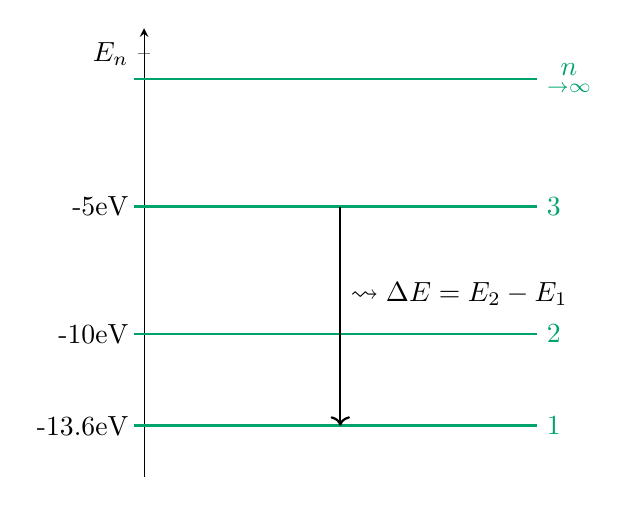
\begin{tikzpicture}
        \begin{axis}[
                xlabel={$n$}, ylabel={},
                xmin=-1, xmax=10, ymin=-15.6, ymax=2,
                xtick={0},
                xticklabels={},
                ytick={1,-5,-10,-13.6},
                yticklabels={$E_n$,-5eV,-10eV,-13.6eV},
                axis y line=left, axis x line=none, axis lines=middle
                ]
                \draw[jade,thick] (-0.2,0) -- (8,0) node[right]{$\underset{\to\infty}{n}$};
                \draw[jade,thick] (-0.2,-5) -- (8,-5) node[right]{$3$};
                \draw[jade,thick] (-0.2,-10) -- (8,-10) node[right]{$2$};
                \draw[jade,thick] (-0.2,-13.6) -- (8,-13.6) node[right]{$1$};
                \draw[black,thick,->] (4,-5) -- (4,-13.6) node[above right,midway]{$\leadsto\Delta E=E_2-E_1$};
        \end{axis}
    \end{tikzpicture}

\end{document}


